% Slides for 2024-04-22
% To create a slide, use the following:


\begin{frame}{Summarize Changes}
    \begin{itemize}
        \item All projects are now done
        \item fixed posts not appear in project updates
        \item fixed 403 error on projects
    \end{itemize}
\end{frame}

\begin{frame}{Lighthouse report for http://e4e-dev.ucsd.edu/acoustic-species-identification/}
    \centering
    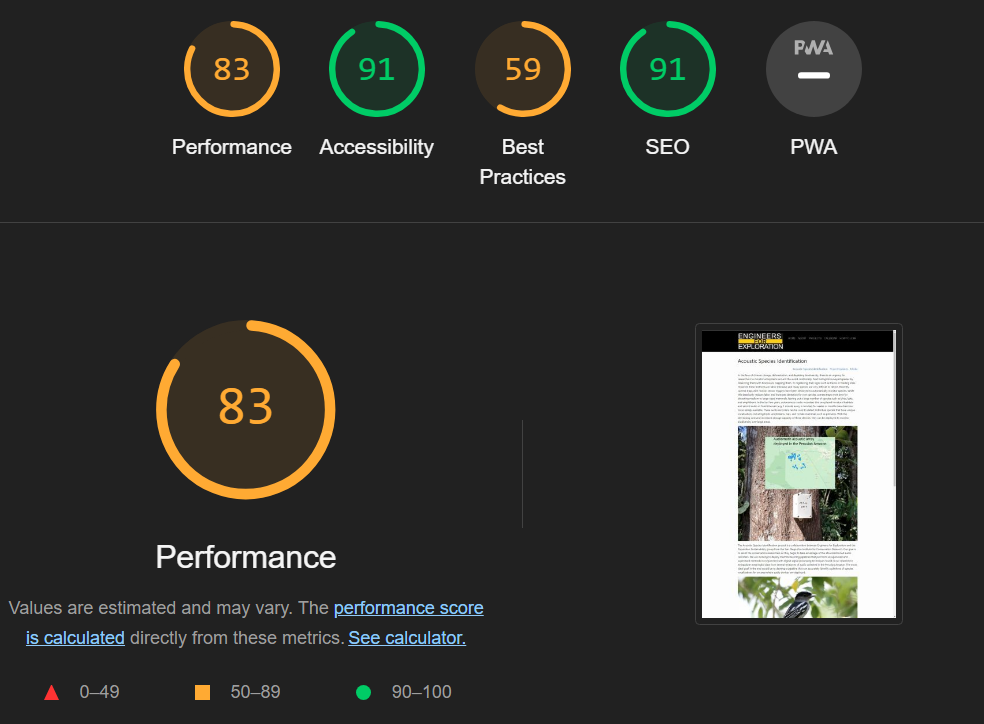
\includegraphics[height=0.7\textheight,width=0.7\textwidth,keepaspectratio]{./images/ligthouse.png}
\end{frame}

\begin{frame}{Lighthouse report for http://e4e-dev.ucsd.edu/acoustic-species-identification/}
    \begin{itemize}
        \item looking good! Original site gets 77
        \item Issue with third party cookies
        \item youtube + google api
        \item http not https (dev site)
        \item Performance issues with images
    \end{itemize}
\end{frame}

\begin{frame}{Dev site is working}
    \begin{itemize}
        \item  \href{http://e4e-dev.ucsd.edu/}{http://e4e-dev.ucsd.edu/}
        \item Seeking feedback, please look
        \item only through UCSD wifi/VPN
    \end{itemize}
\end{frame}



% To create a slide with a graphic:
% 1. Add the graphic to this folder (named picture.png)
% 2. Use the following:
% \begin{frame}{TITLE}
%     \centering
%     \includegraphics[height=0.7\textheight,width=0.7\textwidth,keepaspectratio]{picture.png}
% \end{frame}

% To create a slide with two columns, use the following:
% \begin{frame}{TITLE}
%     \begin{columns}
%         \begin{column}{0.5\textwidth}
%             COLUMN 1 BODY
%         \end{column}
%         \begin{column}{0.5\textwidth}
%             COLUMN 2 BODY
%         \end{column}
%     \end{columns}
% \end{frame}
